\section{Algorithms \& Data Structures}

In this section, there will be analyzed several algorithms in the program, by going in depth with how they were implemented, and how they hold up to algorithms with similar functionality, by comparing their time complexity and memory usage.

\subsection{KDTree} \label{KDTree}
One of the most important parts of making a performant cartography application is to keep the loading and drawing time of the map as low as possible. To achieve this we can eliminate the need to draw unnecessary parts of the map. Such as elements outside of the user's viewpoint or elements that would be too small to be worth drawing. This is where k-dimensional trees become a great utility. K-dimensional trees, or KDTrees, is a data-structure that organizes the dataset such that getting a specified point in space or a multitude of points does not require the computer to read through every datapoint in the dataset.\cite{KDTree} We wish for a data-structure that reads through the smallest amount of data for a correct result. In other words we need the data structures' time complexity to be smaller than O(n), where n is the number of all points of the map.\newline

There are two ways of illustrating a KDTree. One way of illustrating, is to demonstrate the structure of the code, where one can see that the structure is based on a binary tree. This is because of the nature of a KDTree, where every layer of the binary tree switches from the x-axis being the key to the y-axis. This means if a node is being inserted, it compares its values to the tree's value based on the current layer. Therefore in the first layer it compares only the x-values and travels to the right if it is higher, and left if it is lower. An example of input is the yellow circle in figure \ref{KDTree/structure}. 
\begin{figure}[ht]%
  \centering
  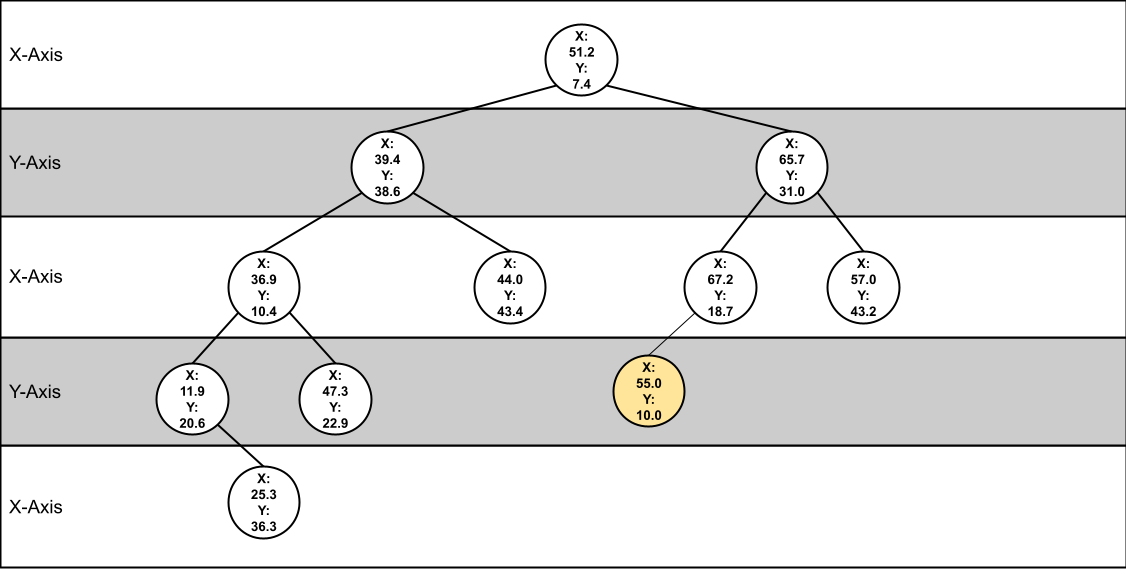
\includegraphics[width=12.5cm]{docs/material/KDTree structure.png}%
  \caption{\centering Demonstration of a KDTree with the structure of a binary tree }\label{KDTree/structure}%
\end{figure}\\
Another way of demonstrating a KDTree is through the inserted node's physical position in a 2 dimensional space. Where every layer is a “cut” in space, such that every child node is either one side or the other. The cut is made alternately in the x-axis and in the y-axis. As seen in the “root” node (marked in the white layer in figure \ref{KDTree/structure}), it has a cut in the x-axis.
\begin{figure}[ht]%
  \centering
  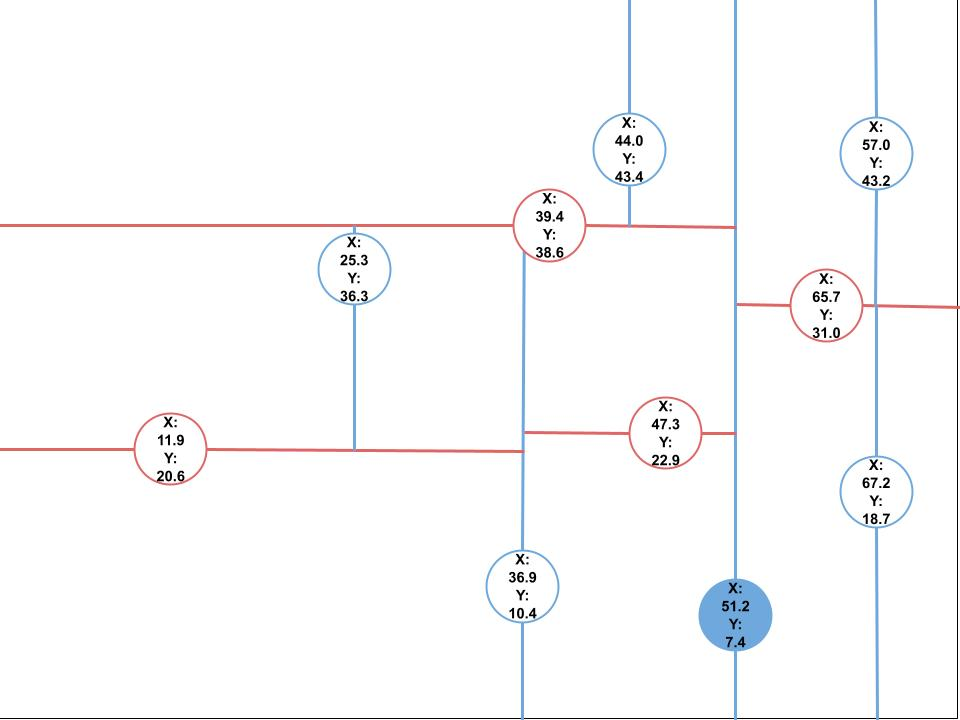
\includegraphics[width=10.5cm]{docs/material/KDTree Visuals.jpg}%
  \caption{\centering Demonstrates how a KDTree partitions segments in space }\label{KDTree/demo}%
\end{figure}\\
The need for a spatial data structure is to cull the unneeded parts of the dataset to only use the data points within the viewpoint of the user. Thus the KDTree is chosen, since it implements a range() function that only returns data points within a specified rectangle on the map, according to the viewpoint. The use of a KDTree also implements a nearest() function that finds the nearest point from an arbitrary point. This can be useful for the user to be able to place points on the map and get information about the nearest point, such as addresses and its coordinates. However we did not get the feature to work through the KDTree, which means that we have made a separate component to find the nearest point.
\newline
We instead made the choice to look through every point in the dataset to find the nearest point. This was done because of time savings, as we had struggled to get the nearest function to work through the KDTree, and we did not have any disposable time left. The choice did not decrease the performance for every frame rendered, because we only used the nearest function to find the nearest road of a point. For example when going from an address, which is a building in the .OSM files, to a road that can be used in pathfinding between two points, which is acceptable as it does not happen every frame.
\newline
When calling the range() function on a 2 dimensional KDTree we get everything within the specified range, but as we implemented hierarchies that only show a specific level of detail (LOD), it would be more efficient to incorporate this hierarchy in the KDTree. This is where a 3 dimensional KDTree would be able to integrate LODs by placing the hierarchy in the third dimension. Which makes the range() function only return data within the specified rectangle and within the LOD group, specified by the zoom level.
\newline
The time complexity is the most important part of KDTrees. We are mostly interested in the time complexity of the range() function as it is called every updated frame. If we analyze the complexity of the function we get an average of O(log(n)) and in the worst case O(n), which is greater than manually checking if a point is within a rectangle for all points on the map, which would be an average time complexity of O(n). This is because of the inherited behavior of a KDTree, where the data is  sorted according to their position. Other than the range() function, we also use the function insert() when inserting a point into the KDTree. This function has a time complexity of O(log(n)) in the best case and in the worst case O(n), but as we only insert elements at the start of the map this does not impact our frame time.
\begin{table}[ht]
  \centering
  \begin{tabular}{ c|c|c }
   \textbf{Function} & \textbf{Average Time Complexity} & \textbf{Worst Time Complexity}\\
   \hline
   \code{range()} & $\Theta(\log(n))$ & $O(n)$ \\
   \code{insert()} & $\Theta(\log(n))$ & $O(n)$ \\
   Search through every datapoint & $\Theta(n))$ & $O(n)$ \\
  \end{tabular}\\
  \caption{\centering Table over time complexities for KDTree}\label{KDTree/timeComplexity}
\end{table}
\subsection{Trie} \label{Trie}
Trie is a data structure for storing strings, which provides a convenient way to search for the different stored strings. It is set up in a ‘tree’ structure, with each node of the tree being a single character. When a string is inserted into the trie, every character is, one by one, put into a node, and as the following set into a child of said node. If a node of said character already exists as a child of the current node, no nodes will be created, and the iteration continues. \cite{AlgoBook/5.2}
\newline
As an example, you could add the strings “stringone”, “stringtwo” and “string” to an empty trie, in that order. First you would start with the root node, which is empty. You then check the first letter of the string, which is “s” in this case. You search in the “branches” hashmap of the empty root node, and see if it already contains the character. If it does not, it creates a new node, and adds it to the hashmap. It then changes the current node to the new node, and repeats the process. When the last character is reached, the node is marked as an end node. On to the second string, “stringtwo”. It would again start off in the root node, and check the branches for any characters matching the first character. In this case you would find it. Instead of creating a new node, it simply sets the current node to be referencing the node containing “s”. It then searches that branch to find any matching characters for the second character, and so on. This repeats until the second “t” (stringtwo) is reached, which is not in the branches of the “g” node. A new node containing the character is then created, followed by two new nodes, the last of which is designated as an end node. As for the string “string”, it will start the same way as the other two, but when it gets to “g”, it will then just mark that as an end node. An end node can still have branches, as it just means that it qualifies as a valid search input.
\newline
Searching in a trie works in almost the same way as inserting. When trying to find a specific string, the first character is searched for in the branches of the root node. If found, this process repeats until an end node is reached, which is a possible answer to the search. In this particular program we are mostly interested in getting a list of search results that fit into what is currently searched for. If no nodes in the branches match the specified character, it would indicate that the string that is searched for is not in the trie.
\begin{figure}[ht]%
  \centering
  \subfloat[\centering Flowchart over Trie algorithm]{{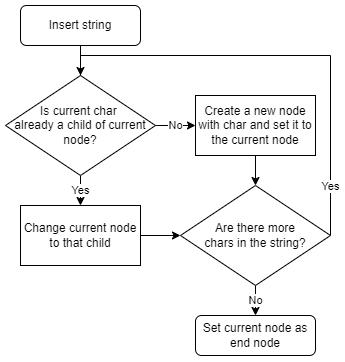
\includegraphics[width=8.25cm]{docs/material/trie flowdiagram.png} }}\label{Trie/flowdiagram}%
  \subfloat[\centering Example of how the Trie data structure changes as more strings are inserted]{{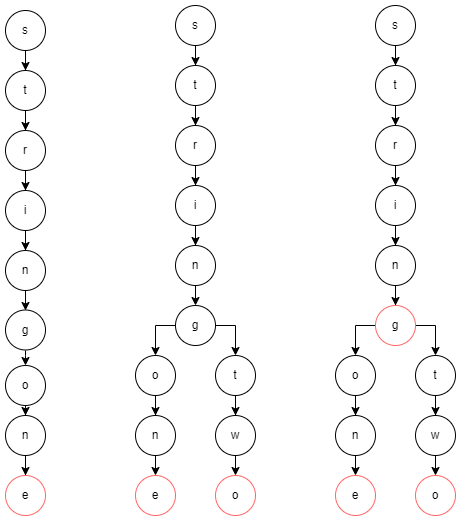
\includegraphics[width=8.25cm]{docs/material/trie demo.png} } \label{Trie/demo}}%
  \caption{Illustrations of Trie algorithms}
\end{figure}
\subsubsection{Why would we use Trie?}
It was a requirement for the program to be able to handle searches for an address as a single string, and for it to be able to “handle ambiguous user input appropriately, e.g., by displaying a list of possible matches.”.\ref{Trie/demo} A way to do this would be to simply store all the addresses in a hashmap, and use regular expressions to separate the different parts of the address. An algorithm, Levenshtein distance, could be used to approximate what strings the user could have meant instead of their exact input. This is mostly useful in cases where the user misspelled the input, in which case the program would ideally suggest the actual address they were searching for.\\
An alternative for this solution is the trie. A trie allows for the program to make suggestions on what address the user might be searching for. When the user then tries to find a specific address, the program only has to search through the hashmap of the house numbers connected to the specific road, instead of a 
hashmap of every single address.
\subsubsection{Trie Implementation}
\begin{wrapfigure}{r}{0.5\textwidth}
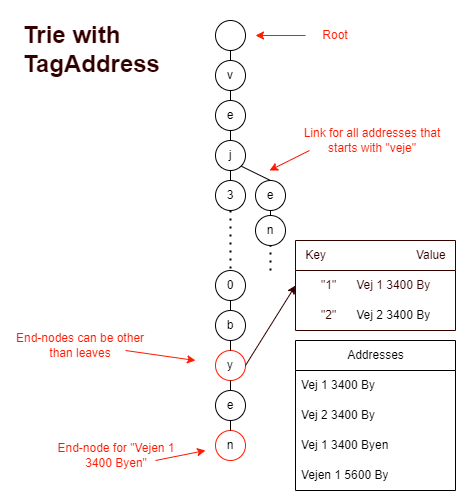
\includegraphics[width=0.9\linewidth]{docs/material/Trie Diagram.png} 
\caption{Example of Trie data structure with fictional addresses}\label{Trie/implementation}
\label{fig:wrapfig}
\end{wrapfigure}
When a string is added to the trie, all of the spaces are removed. This means that the strings “Hvidovrevej” and “Hvidovre vej” would be treated the same. 
We decided that we wanted to store the addresses in the format of house number, 
postcode and city, for instance “Hvidovrevej 2650 Hvidovre”. The spaces are then removed, and everything is made lowercase. What is inserted into the trie will thus be “hvidovrevej2650hvidovre”. All end nodes have a hashmap which contains the different house numbers connected to the road, city and postcode. In the case just mentioned, the end node would be the final “e” in “hvidovre” (the hvidovre after the postcode). That node would then contain a hashmap which contains the TagAddress objects corresponding to the house numbers present on Hvidovrevej 2650 Hvidovre. This makes searching for an address a lot faster, than trying to go through a whole hashmap of addresses. The different possible addresses are added to a list, which is displayed in the search bar. Only the street, postcodes and city names are shown initially, but after a specific street has been chosen by the user, the different house numbers are then displayed, again allowing the user to pick the specific address they desire.\\
A remove method was not implemented in the Trie class as it was deemed unnecessary in the circumstances of the program. 
\newline
Implementing Trie into the system, there is a search bar which allows the user to type in whatever they desire. Whenever the user types in a new character, the program will search through the Trie tree, which contains all possible addresses for the given map.
\newline
If the user would type “hvidovre” into the search bar, Trie would look up at most 5 different suggestions for addresses that start with the given input. The user will now see that 2 suggestions pop up. These are TrieNodes set as an end-node, which each contain a hashmap, linking house numbers to real addresses.
If the user were to click on “Hvidovrevej, 2650 Hvidovre”, the user would get all the endnode’s values. 
Now the user can click on whichever address they desire, and searching will hereby be complete. 
\newline
If they were to continue writing an address instead of clicking on “Hvidovrevej, 2650 Hvidovre”. The program will detect that only one TrieNode can be found in the Trie tree. Since this is the case, the program will then lookup house numbers as the previous example.
\subsubsection{Memory and performance}
Trie will be stored into the heap as soon as Bornholm has been read. The size of Trie does not change during runtime afterwards.\\
The following benchmarks are performed on a pc with intel-i7 6700 processor and 16 GB 3200 MHz ram.
\begin{table}[ht]
  \centering
  \begin{tabular}{ c|c|c }
   \textbf{Object} & \textbf{Count of instances} & \textbf{Size}\\
   \hline
   Heap used for Bolmholm & $\sim7.5$ million & $344.118$ kB \\
   TrieNode & $\sim27.000$ & $868$ kB \\
   TCharObjectHashMap & $\sim27.000$ &  $1.735$ kB\\
   Key, value pair in Hashmaps & $\sim60.000$ & $1.920$ kB \\
   HashMap & $\sim27.000$ & $1.296$ kB\\
   Sum of Trie algorithm & $\sim141.00$ & $5.819$ kB ($1,69\%$)
  \end{tabular}\\
  \caption{\centering Memory usage of Trie, compared to the rest of the program, which is the entire heap of Bornholm}\label{Trie/memory}
\end{table}
\begin{table}[ht]
  \centering
  \begin{tabular}{ c|c }
   \textbf{Operations} & \textbf{Avarage running time}\\
   \hline
    Running time for finding five address suggestions & $\leq 1$ms\\
    Inserting all Addresses for Bornholm into Trie & $\sim 100$ms \\
  \end{tabular}\\
  \caption{\centering General operations for Trie}\label{Trie/operations}
\end{table}
The results on memory and performance suggest that Trie works for the program. 
\newpage
Optimizing the data structure would only be able to improve memory with small per-milles. Any larger mathematical sequences such as getting suggestions or inserting all addresses into Trie, is not slower than instantaneous. \\
It can thereby be concluded that Trie’s functionality does not get in the way of the larger systems performance and memory usage. If the program were to handle larger maps, Trie would still be rather effective, due to its time complexity.
\begin{table}[ht]
  \centering
  \begin{tabular}{ c|c }
   \textbf{Operations} & \textbf{Average running time}\\
   \hline
    Running time for finding an address suggestion & $\Theta(\log n)$\\
    Inserting all addresses & $\Theta(n)$ \\
  \end{tabular}\\
  \caption{\centering Time complexities in Trie, where $n$ is the number of addresses}\label{Trie/timecomplexity}
\end{table}
\subsubsection{Improvements}
The implementation of Trie did not allow for addresses to be found without entering the whole string. This prevents it from being used in the case that you want to find an address based on something else, like position. This resulted in the need for saving the addresses in some other place, if the program were to support such cases.\\
It also does not consider spelling mistakes made by the user. To fix this, a merge between the Levenshtein algorithm and Trie would be beneficial. Simply whenever the user types in a street, city or postcode in and it does not give any results. The Levenshtein algorithm will be used to find any possible string that is closest to the user’s input.
\subsection{Minimum Priority Queue}
The Minimum Priority Queue (PQ) has two is being used in Minion Maps pathfinding and in layer sorting. The priority queue is a heap-ordered complete binary tree, where the root will be the minimum value, and the following will continuously be the next smallest value.\\
The Priority queues in Minion Maps, have been inspired from SedgeWick and Wayne’s book on Algorithms, and implements many of the features from the book.
The priority queue sorts with the \code{swin()} and \code{sink()} operations, meaning that values within the tree exchange index position with one another, up and down they go, until their parent has a smaller value and their children a larger value (vice versa for MaxPQ).
\subsubsection{Priority Queue in Pathfinding}
In Minion Maps, The pathfinding algorithm Dijkstra is implemented with the use of a modified Minimum Priority queue, called an Index Minimum Priority Queue (IndexMinPQ). The modified priority queue supports the same methods as the normal priority queue, but also has the methods decreaseKey() and increaseKey(). These operations support updating the priority of a key at a specified index. To implement this in Minion Map, we maintained a hash-map where each key represents a key-value pair’s key and points to the index of the key. We then update the value at the specified index and reposition the current element based on its priority, and then update the index value in the hash-map accordingly. This ensures that the two methods have a time complexity of $O(\log{n})$.\cite{PQ/geeksforgeeks} This is useful in the case of dynamically changing the priority of an element, and that comes very much into play when we update the best candidate vertex in the priority queue.\par
The priority-value of a given element can be changed, depending on what the search-term the user selects. The search-term changes if the priority queue should be prioritized by the distance (shortest path) or time (fastest path).

\subsubsection{Priority Queue in Layers}
\begin{figure}[ht]%
  \centering
  \subfloat[\centering Example of layering Rønne in different type, where a type with the smallest value is behind everything else]{{\includegraphics[width=7.45cm]{docs/material/Good Layers of Rønne.png} }}\label{PQ/goodLayers}%
  \subfloat[\centering If the island of Bornholm were to be drawn in front of everything else (building, water etc.)]{{\includegraphics[width=8.85cm]{docs/material/Bad Layers of Rønne.png} } \label{PQ/badLayers}}%
  \caption{Illustrations of layering of Rønne}
\end{figure}
\newpage
\begin{wrapfigure}{r}{0.44\textwidth}
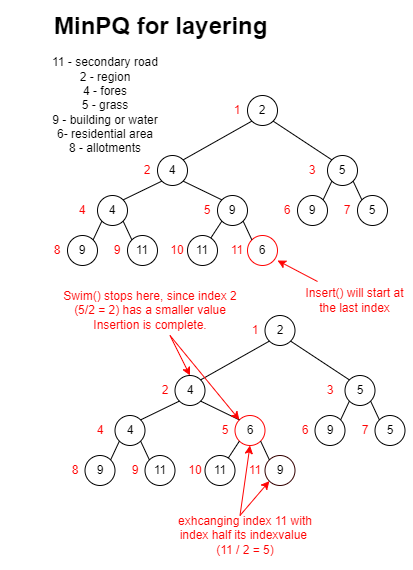
\includegraphics[width=0.9\linewidth]{docs/material/Insert in minPQ.png} 
\caption{Inserting a value into the Minimum priority queue}\label{PQ/insert}
\label{fig:wrapfig}
\end{wrapfigure}
When drawing maps, it can be useful to define in what order, different types of polygons and lines should be drawn first. Otherwise, when reading an .OSM file, there would be a risk of drawing large polygons such as the island of Bornholm above everything else on the island. Instead, it is necessary to ensure that the island of Bornholm gets drawn \textit{first} where the following polygons will be drawn afterwards, thus, polygons such as buildings will be \textit{on top} of Bornholm.\\
The solution to this problem would be to \textbf{assert a value to a \textit{type} of polygon or line}, which a priority queue can use to compare its data. When obtaining a whole list of objects that should be drawn on the screen. All instances will be redirected over to the minimum priority queue with the insert() method. Here, an object will be put as the last index of the queue, and will begin to “swim” upwards appropriately using its \textbf{layer value}, until its parent’s value is smaller than itself. 

\begin{wrapfigure}{r}{0.44\textwidth}
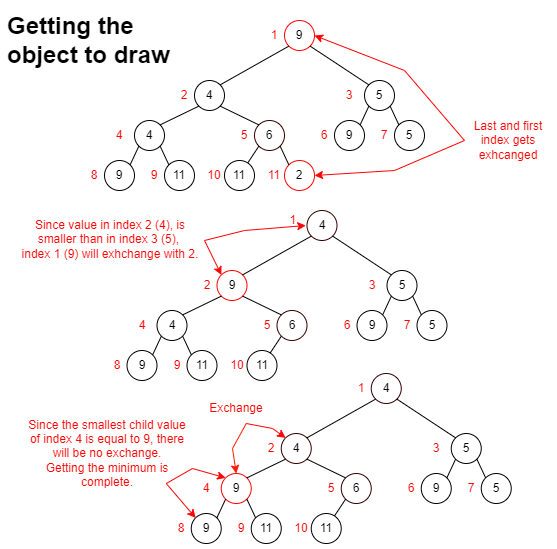
\includegraphics[width=0.8\linewidth]{docs/material/RemoveMin.png} 
\caption{Deleting the minimum value of the MinPQ}\label{PQ/remove}
\label{fig:wrapfig}
\end{wrapfigure}
Once every object to be drawn has been inserted, the minimum object will be deleted from the queue and will be drawn. This happens by exchanging the root (the minimum value) with the last index. Once this has been done, there is a good chance that the new root is misplaced. Here the sink() method will be used. Which exchanges the given index with one of its children, preferably the child with the smallest value, until none of its children is smaller than the value to sink.
\newpage
\noindent
\subsubsection{Memory and performance}
An instance of a MinPQ has
\begin{itemize}
\setlength{\itemsep}{0.1em}
    \item An array of the given type, the size in memory the chosen type’s size time with the length of the queue.
    \item An integer, which is the amount of objects stored on the pq.
\end{itemize}
The size of the array on this project’s instance is precisely based on the amount of lines and polygons to draw.
And an integer is only 4 bytes.
\begin{table}[ht]
  \centering
  \begin{tabular}{ c|c|c }
   \textbf{Object} & \textbf{Count of instances} & \textbf{Size}\\
   \hline
   Heap used for Bolmholm & $\sim7.5$ million & $344.118$ kB \\
   TagWay & $\sim79.000$ & $3.792$ kB \\
   Sum of MinPQ for layering (worst case) & $\sim79.000$ & $\sim316$ kB $(0.09\%)$ \\
  \end{tabular}\\
  \caption{\centering Table of Memory usage with MinPQ compared to the entire heap, while running Bornholm.
}\label{PQ/memory}
\end{table}
\newline
Although each TagWay takes up 48 bytes. MinPQ will only take up 4 bytes per TagWay, since TagWay is a reference type, the array will store references to an object, which takes up 4 bytes per reference. 4 Bytes * 79,000 = 316 kB.
\newline
The following benchmarks are performed on a pc with intel-i7 6700 processor and 16 GB 3200 MHz ram.
\begin{table}[ht]
  \centering
  \begin{tabular}{ c|c }
   \textbf{Operations} & \textbf{Average running time ($\sim 5.000$ objects})\\
   \hline
    Inserting all ways into the MinPQ & $\leq 1$ms\\
    Obtaining and deleting the entire MinPQ & $\sim 2$ms \\
  \end{tabular}\\
  \caption{\centering Operations for Minimum Priority Queue}\label{PQ/operations}
\end{table}
When running Bornholm, it is on average 5,000 lines or polygons, no matter where you zoom or pan, and looking at these operation times, makes it clear that using a minimum priority queue for layering, takes almost no resources on the computer, considering the other parts of the program.
\subsubsection{Comparison with alternative sorting-algorithms}
If we were to consider other sorting methods. No other alternative (from the book) seems to work more efficiently, as far as our reasearch brought us. MinPQ, which is arguably similar to heapsort (since heapsort is built from PQ’s \code{delMax()} method), will use $O(N \log N)$ time for sorting all TagWays, where $N$ is the number of TagWays.\cite{AlgoBook/2.5} This process is almost identical to deleting the minimum value in MinPQ until there are no elements left. 
Sorting-algorithms similar to MinPQ’s sorting running time would be mergesort, quicksort and 3-way quicksort. The problem with all these three algorithms is their extra use in memory. Heapsort is the only one of these four algorithms, of which extra space is a constant size (Object header, padding, size integer), while the others use at least extra space of $\lg N$.\cite{AlgoBook/2.5} This extra memory can be found in the stack whenever the algorithm sorts, since quicksort and 3-way quicksort are recursive algorithms, whereas heapsort is just iterative. 
\subsection{Pathfinding}
Minion Maps implements a edge-weighted digraph for representing the road network, with support for the A* pathfinding algorithm.\par
In order to figure out what the best way to represent the road network of Minion Maps, and give the user the ability to find the shortest route. We will need to discuss the use of the directed edge-weighted graph or edge-weighted digraph data structure and pathfinding algorithms. 
\subsubsection{Edge-Weighted Digraph}
To make a good representation of a real life road network, we need to take multiple considerations into account. How do we represent roads, intersections, one-way streets and more as a data type? In Minion Maps, we have chosen to use a edge-weighted digraph to address all of these considerations.\par 
A directed graph (or digraph) is a set of vertices and a collection of directed edges that each connects an ordered pair of vertices. In the case Minion map the directed edges are weighted, to help distinguish what road is faster to go through. In the terminology in the case of Minion Maps, the vertices are a TagNodes and the weighted edges are a pair of TagNodes with distance as the weight. The digraph in Minion Map uses the adjacency-list representation, where we have a vertex-indexed array of lists which contain the vertices connected by weighted edges. The representation can be constructed and take up $\Theta({E+V})$ time and space, where $E$ is the number of edges and $V$ is the number of vertices. 
The actual data structure in the adjacency-list is a list of links to weighted edges containing the references to other weighted edges. 
\begin{figure}[ht]%
  \centering
  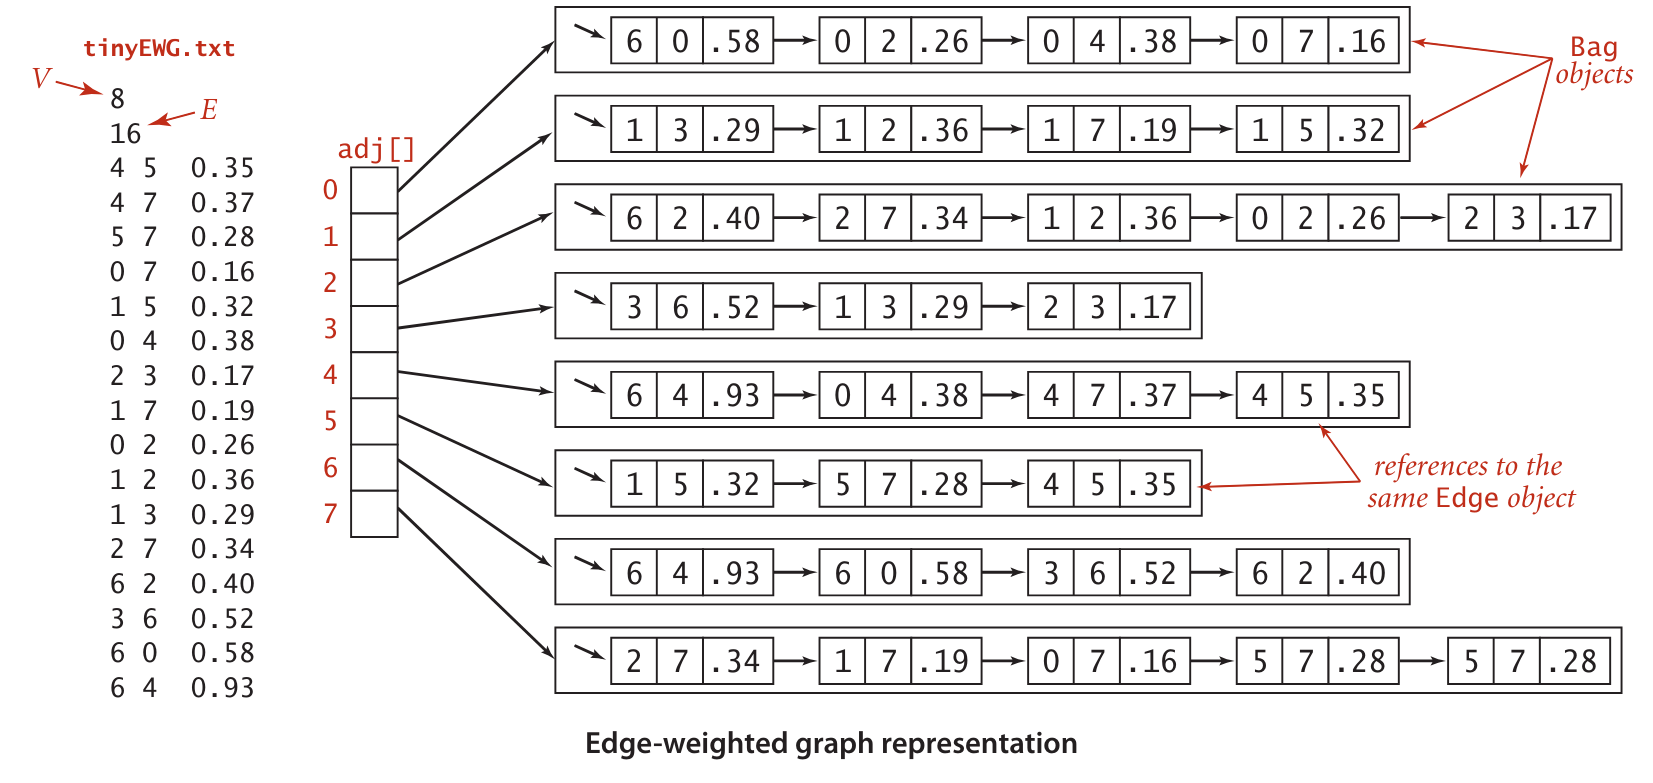
\includegraphics[width=10.5cm]{docs/material/edgeWeightedGraphRepresentation.png}%
  \caption{\centering Edge-weighted graph of the adjacency-list representation\cite{AlgoBook/4.3}}\label{graph/AdjList}%
\end{figure}\\
When implementing the Edge-Weighted digraph in Minion Maps, we implemented the vertex-indexed array as a TreeMap instead of a normal list. This is to achieve a search time of $O(V \log E)$ time instead of getting a search time of $O(V+E)$ when using an array representation.\cite{graph/geeksforgeeks} The reason why we get sequential search time on the array representation, is because the vertices are stored unordered and as objects and we thereby do not know their index in the array. We therefore use a TreeMap that implements a natural ordering of its keys and use a balanced Red-Black search tree to gain a search time of $O(V \log E)$ in the worst.
\subsubsection{Dijkstra \& A*}
Dijkstra is a famous pathfinding algorithm that finds the shortest path between two nodes in a weighted graph. Minion Maps supports both Dijkstra and a variant of Dijkstra called A* (pronounced “A-star”), that uses heuristics to find the shortest path more efficiently. The main mechanism in Dijkstra’s algorithm is to recursively find the best candidate vertex for creating the shortest path from one vertex to another.\cite{Dijkstra} \\
\newpage
\begin{algorithm}
\caption{Dijkstra's Algorithm\cite{Pathfinding/Code}}\label{dijkstra}
\begin{algorithmic}
\\
    \Procedure{Dijkstra}{$G, s$} \Comment{Digraph $G$ and source vertex $s$}
        \State Initialize $Q$ as an empty priority queue
        \State Initialize $d[v]$ to $+\infty$ for each vertex $v \in V[G]$
        \State \textproc{Insert}$(Q, s, 0)$ \Comment{Insert source into queue with distance 0}
        \While{$Q \neq \emptyset$}
            \State $(u, k) \gets \textproc{Delete-Min}(Q)$ \Comment{Extract vertex with minimum distance}
            \State $d[u] \gets k$ \Comment{Update shortest distance to $u$}
            \ForAll{$(u, v) \in E[G]$} \Comment{Iterate over neighbors of $u$}
                \If{$d[u] + w(u, v) < d[v]$}
                    \If{$d[v] = +\infty$} \State \textproc{Insert}$(Q, v, d[u] + w(u, v))$
                    \Else \State \textproc{Decrease-Key}$(Q, v, d[u] + w(u, v))$
                    \EndIf
                    \State $d[v] \gets d[u] + w(u, v)$ \Comment{Update shortest distance to $v$}
                  \EndIf
            \EndFor
        \EndWhile
    \EndProcedure
\end{algorithmic}
\end{algorithm}
Dijkstra keeps track of the distance for all edges between the start $s$ vertex and any given vertex $v$ through the \code{distTo[]}, while simultaneously updating the priority queue with the element's priority-value, which is the distance between the two vertices divided by the speed limit of the road. Dijkstra uses relaxation of an edge $u \rightarrow v$ to test whether the best-known way from $s$ to $v$ is through $s \rightarrow v$, or by going through the edge $u \rightarrow v$. If going though $u \rightarrow v$ is the best way by comparing the edges weights, then update our data structures to indicate that this is the case \cite{AlgoBook/652}. As this is a recursive method, the process starts again with the newly assigned best edge until a route is found from the starting point to the end point. 
\newline
A*  takes a heuristic distance into account when prioritizing the vertices. A* utilizes heuristic values to assert how to prioritize the given vertices. A* takes into account the distance from any given vertex to the end vertex (hScore) and the distance from any given vertex to the start vertex (gScore). A* then prioritizes the vertex with the lowest fScore, which is the addition of the two heuristic distances $fScore = hScore + gScore$\newline
The heuristic of A* can be implemented in different ways and the quality of the heuristic and how to approximate the hScore, can have a big impact on the running time of the algorithm. If the heuristic in theory did not help cutting down the possible branches that the algorithm could search though, we could calculate the time complexity by estimating the amount of vertices the algorithm has explored. Here the time complexity of A* would be $O(b^d)$, where $b$ is the average amount of outdegrees a vertex has, and $d$ is the depth of the shortest path. If the heuristic is well implemented, the heuristic would decrease the amount of outdegrees the algorithms would have to search though.
\newline
The Psudecode for A* would almost be identical as Dijkstra, except when inserting or decreasingKey of the priority queue, the heuristic value is being added on top of current weight.
\begin{table}[ht]
  \centering
  \begin{tabular}{ c|c|c|c }
   \textbf{Algorithm}& \textbf{Function} & \textbf{Average Time Complexity} & \textbf{Worst Time Complexity}\\
   \hline
  Dijkstra & \code{shortestPath()} & $\Theta(E\cdot\log(V))$ & $O(V^{2})$ \\
  A* & \code{shortestPath()} & $\Theta((*b)^{d})$\cite{Stuart&Peter} & $O(b^{d})$
  \end{tabular}
\end{table}
\begin{figure}[ht]%
  \centering
  \subfloat[\centering Illustration of Dijkstra's Algorithm]{{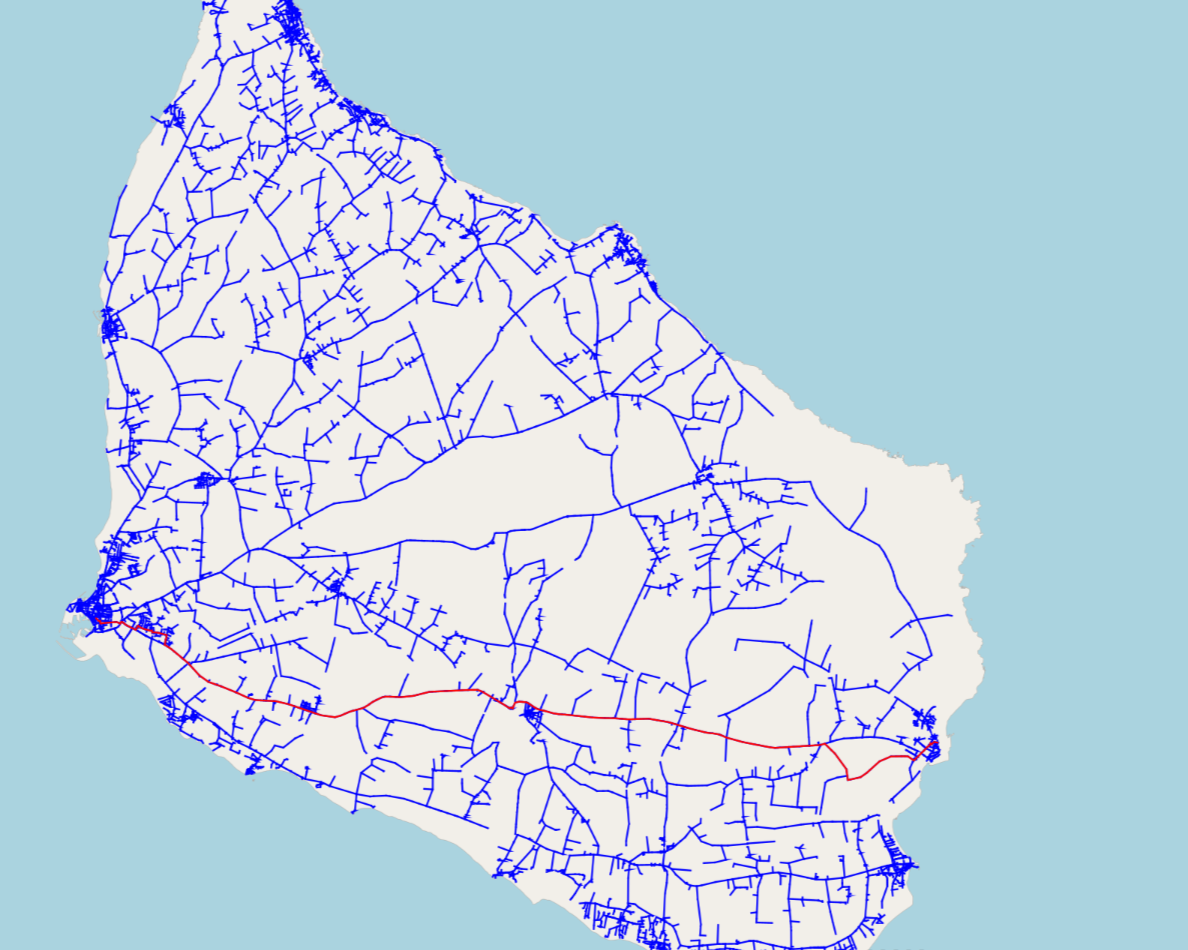
\includegraphics[width=8cm]{docs/material/Pathfinding_Bornholm_Dijkstra.png} }}\label{Pathfinding/dijkstraPic}%
  \subfloat[\centering Illustration of A* Algorithm]{{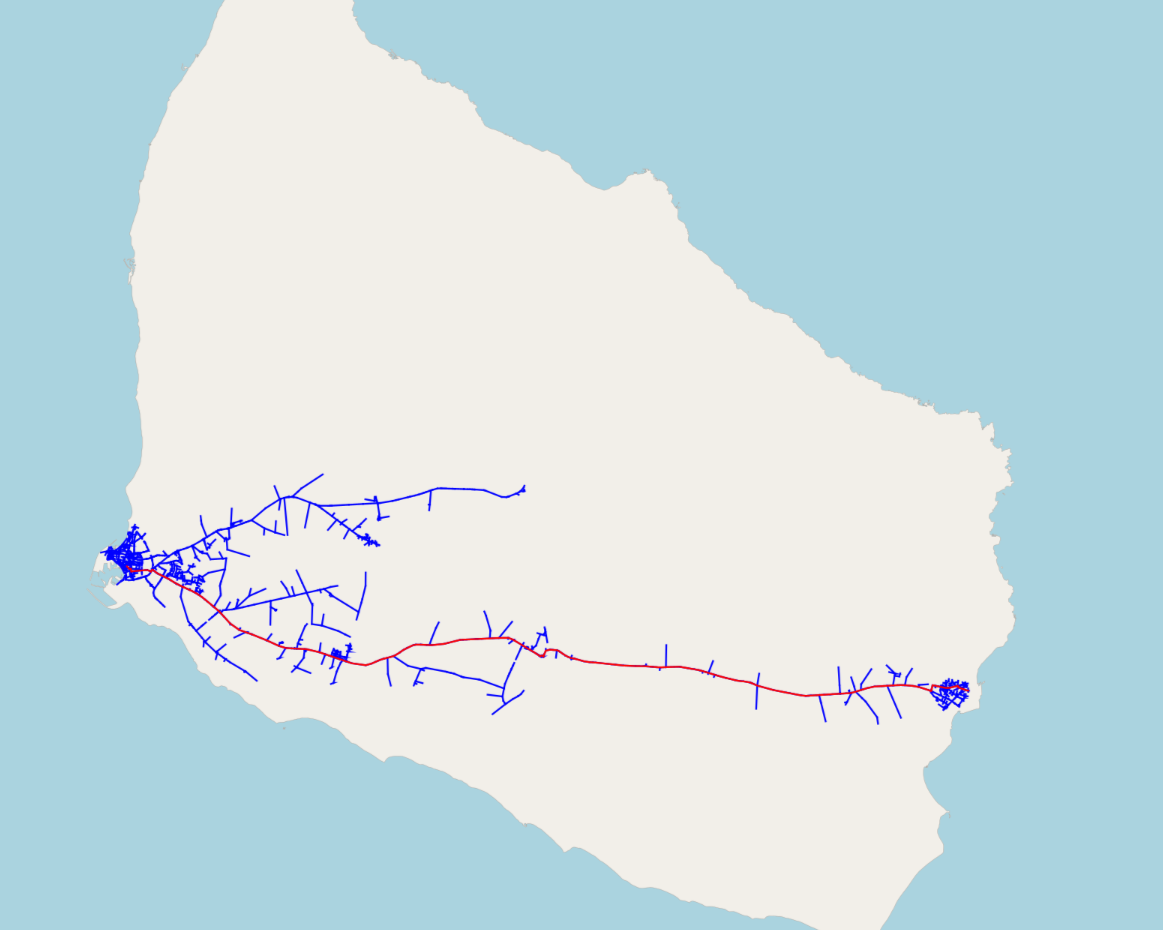
\includegraphics[width=8cm]{docs/material/Pathfinding_Bornholm_A_Star.png} } \label{Pathfinding/A*Pic}}%
  \caption{Illustrations of the Dijkstra and A* pathfinding algorithms in Minion Map, where the red line is the shortest path and the blue is visited paths}
\end{figure}
\newpage
\subsubsection{Douglas Peucker}
An experiment that was attempted was to reduce running time for drawing the map by reducing the amount of points to draw lines to. This could be done with the Douglas Peucker algorithm which iteratively reduces the point between an endpoint and a startpoint. \cite{Douglas/Peucker}

\begin{wrapfigure}{r}{0.55\textwidth}
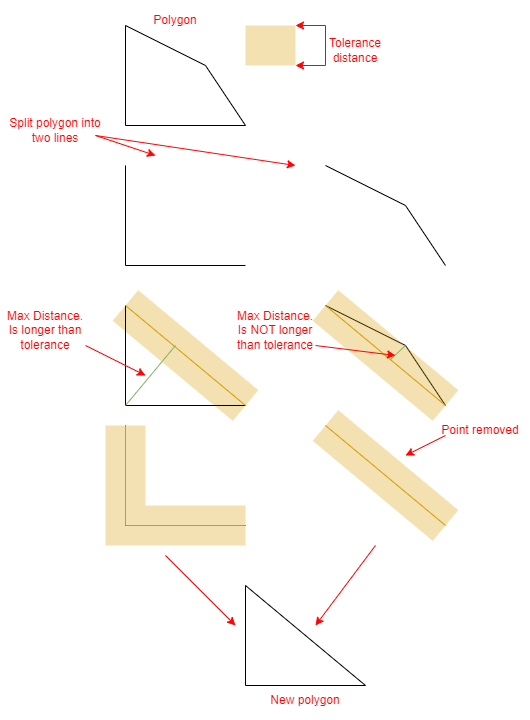
\includegraphics[width=0.68\linewidth]{docs/material/Douglas Peucker.png} 
\caption{ Process for Douglas Peucker over a polygon}\label{DouglasPeucker}
\label{fig:wrapfig}
\end{wrapfigure}
Say there is a line with $n$ amount of points. Then the Douglas Peucker algorithm removes points based on the length of a tolerance distance. At the start of the algorithm. A line is drawn from the startpoint to the end point. Then the point that is furthest away from that line is checked whether it is within the tolerated distance or not. If it is all points except the start and the end point gets removed. Else, this point will be added to the line, and the point that is closest to this line will then be checked. This iteration continues until a point is within the tolerance distance.\\
Douglas Peucker would be implemented by simplifying all polygons and lines based on how far the user zooms out on the map. As the user zooms further out, the tolerance distance would become larger, and thus lines and polygons would become simpler and simpler. This was however not a very optimal idea, as the algorithm would have to run whenever the user would zoom out, and since the amortized time complexity is $O (n \log m)$\cite{Douglas/Peucker}, 
where $n$ is the number of points and $m$ the number of points for the new, simplified line. The algorithm would simply have to handle too many polygons and lines at once, and too often as well. Additionally the algorithm conflicts with the newly structured LinkedList foundation, where each point is chained to the next and its previous, and breaking this chain may require additional calculations. It is possible that there could be a work around, where the linkedlist itself would not be changed, but only some of the points would be marked as drawable. If there was more time to work on the project, Douglas Peucker may be a possible implementation, but due to its many challenges, the algorithm simply was not fitting enough for our problem to be prioritized higher than other algorithms.
\newpage